% -*- coding: utf-8 -*-
\section{Remise en contexte}
\subsection{Pr{\'e}sentation de l'entreprise}
\begin{frame}
  \frametitle{Pr{\'e}sentation de l'entreprise}
  \textbf{SEW Usocome}

  \begin{minipage}{.5\textwidth}
  \begin{itemize}
  \item filiale fran{\c c}aise du groupe allemand \textbf{SEW-EURODRIVE}
  \item usines {\`a} Haguenau, Brumath et Forbach
  \item propose des solutions d'automatisme pour des applications de
    mouvement (moteur {\'e}lectrique, servomoteur..)
  \end{itemize}
\end{minipage}%
\begin{minipage}{.5\textwidth}
  \begin{figure}
    \centering
    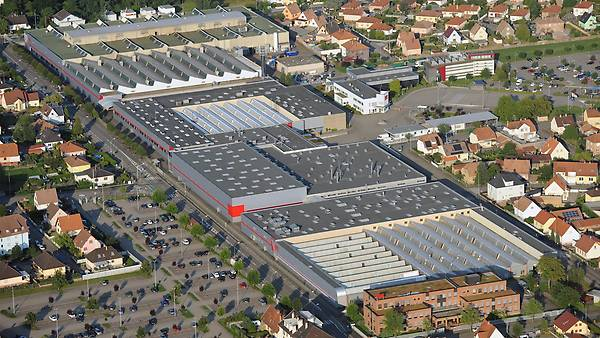
\includegraphics[scale=1,width=0.9\textwidth]{sew_haguenau.jpg}
    \caption{Vue de l'usine de Haguenau}
    \label{fig:sew_haguenau}
  \end{figure}
\end{minipage}
\end{frame}
%
% %%%% --4--%%%%
\subsection{Etat actuel}
\begin{frame}
  \frametitle{Etat actuel}

  Gestion des stocks inexistantes entre les zones de production et de
  stockage et les autres usines.

  \textbf{Probl{\'e}matique~:} Avoir constamment des contenants vides sur
  les zones de production et suffisamment de contenants utiles {\`a} la
  production sur chaque site

  \begin{minipage}{.5\textwidth}
    \begin{figure}
      \centering
      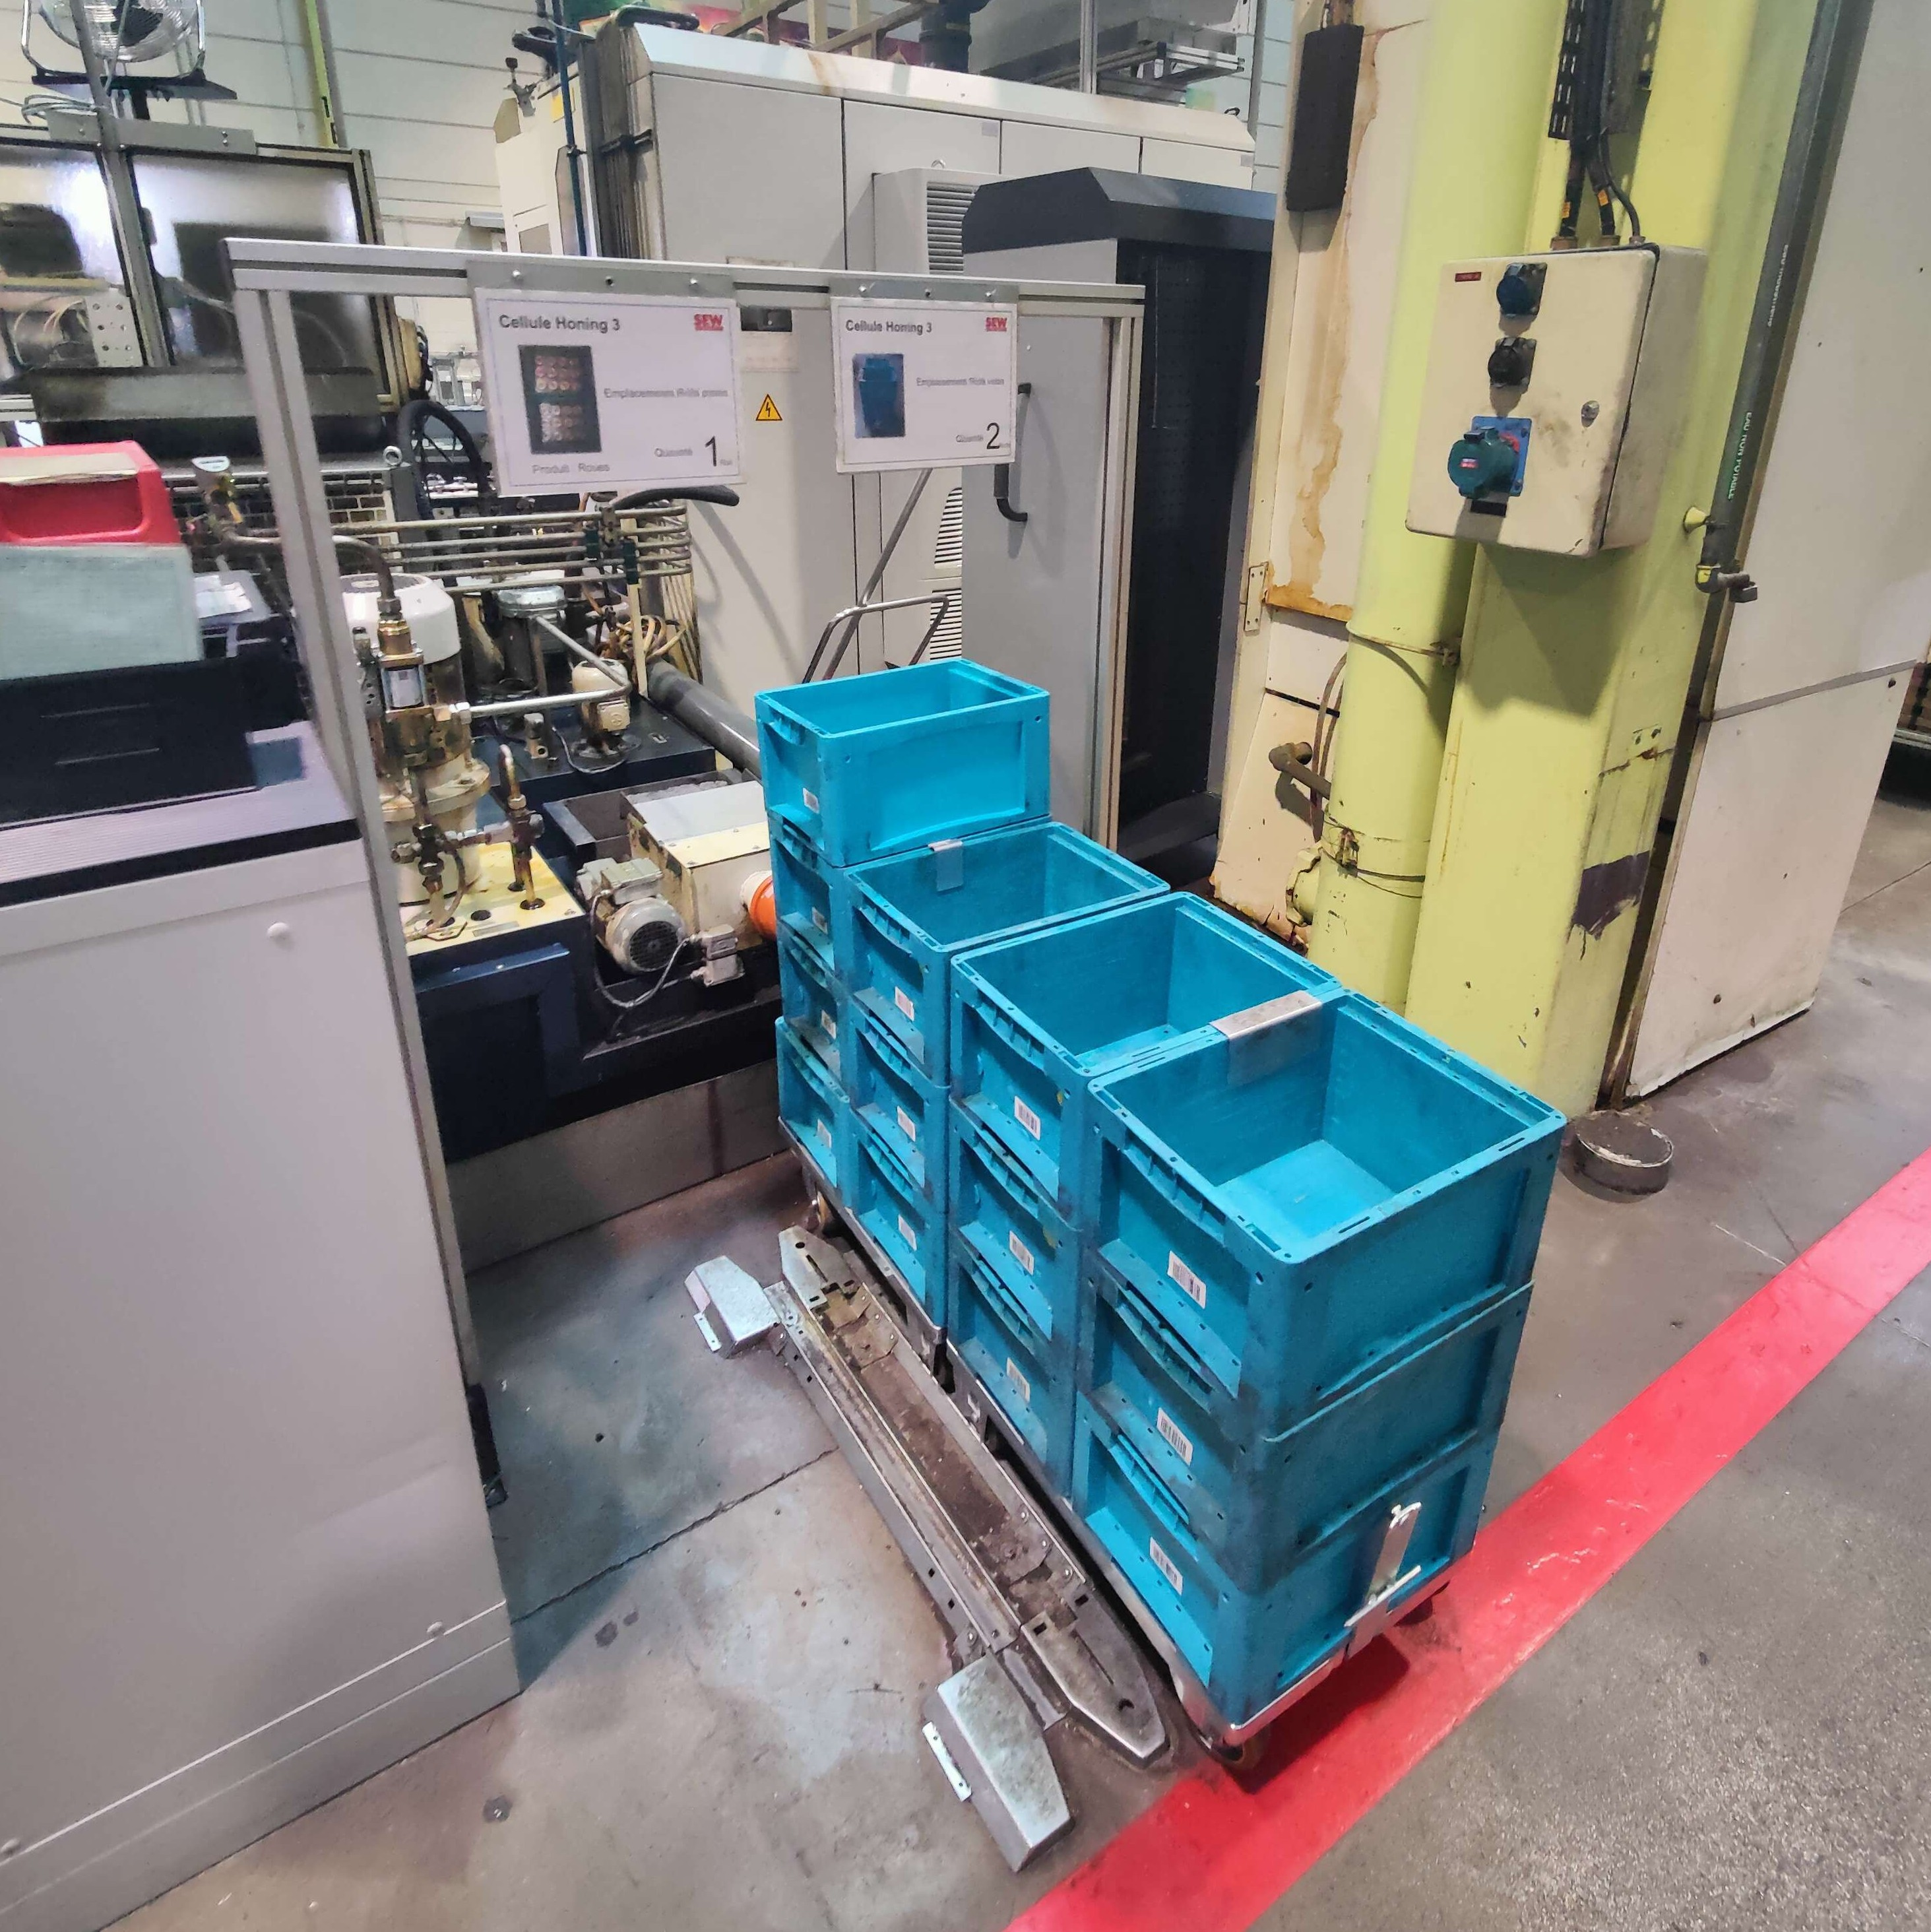
\includegraphics[width=0.7\textwidth, height=0.47\textheight]{sew_production.jpg}
      \caption{Image d'une zone de production d'Haguenau}
      \label{fig:sew_production}
    \end{figure}
  \end{minipage}%
  \begin{minipage}{.5\textwidth}
    \begin{figure}
      \centering
      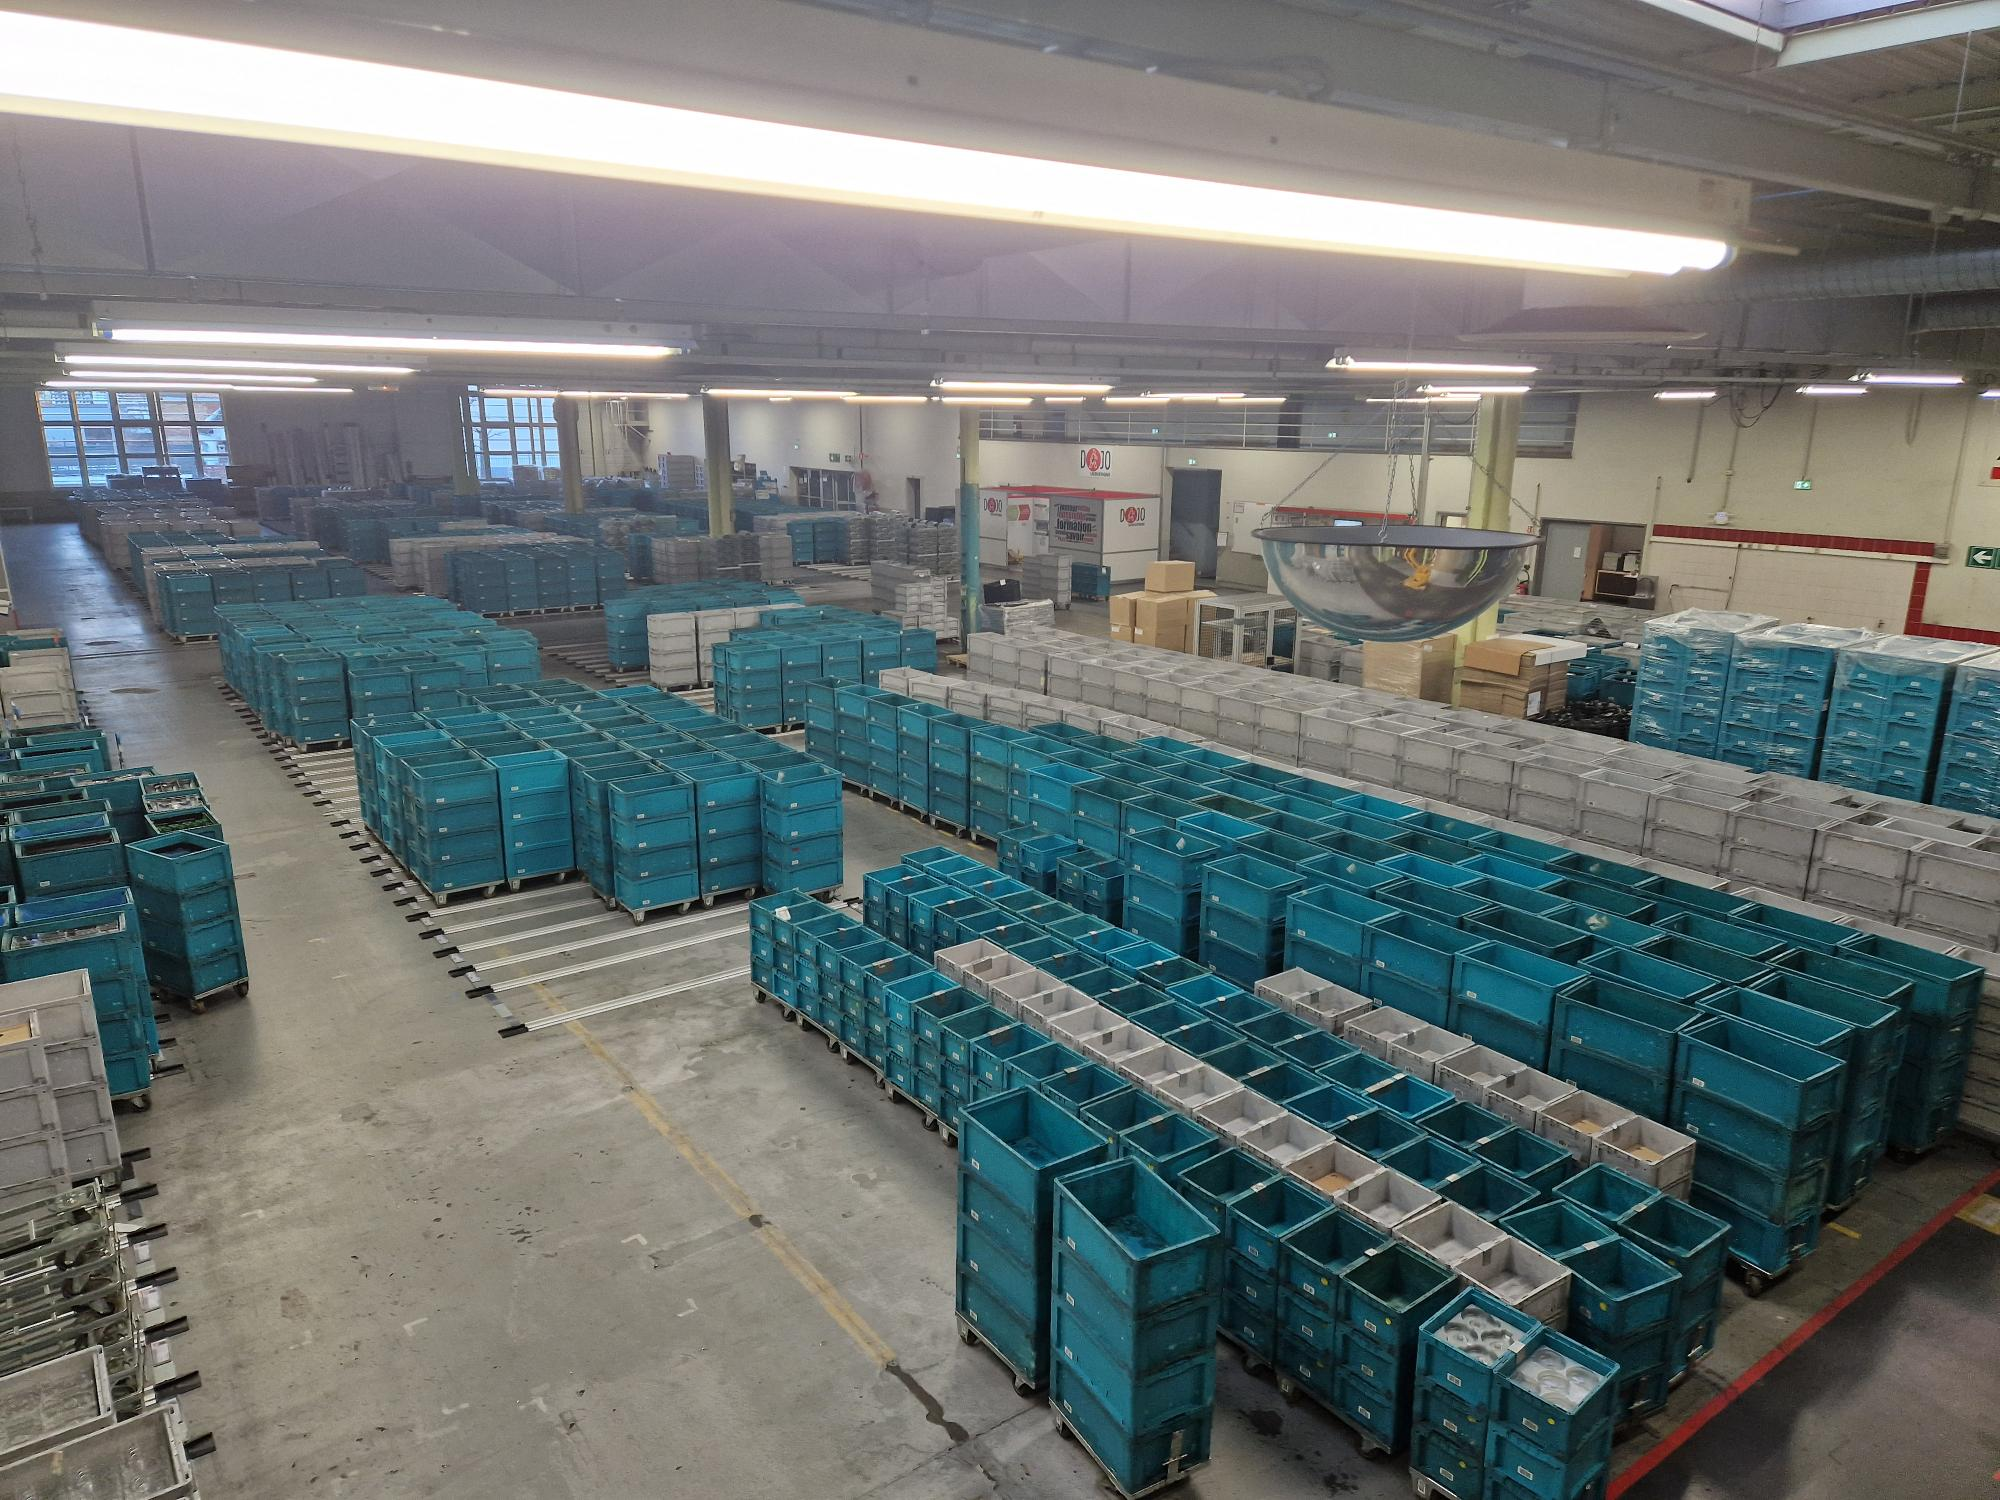
\includegraphics[scale=1,width=0.9\textwidth]{sew_entrepot.jpg}
      \caption{Image de la zone de stockage de Haguenau}
      \label{fig:sew_entrepot}
    \end{figure}
  \end{minipage}
\end{frame}%
% %%% --5--%%%
\subsection{Objectifs du projet}
\begin{frame}
  \frametitle{Objectifs du projet}
  \textbf{Objectif principal~:} Classification et comptage des
  contenants vides

  \begin{center}
    \scriptsize
    \begin{tabular}{|p{3cm}|p{4cm}|p{3cm}|}
      \hline
      Objectifs & Crit{\`e}res & Moyens \\
      \hline
      Acquisition de donn{\'e}es num{\'e}riques & 1. Avoir assez d'images des
                                          diff{\'e}rentes bo{\^\i}tes r{\'e}parties homog{\`e}nement & Utilisation de cam{\'e}ras IP \\
                & 2. Acquisition dans nos locaux et {\`a} SEW & \\
      \hline
      Classification des types de bo{\^\i}tes par apprentissage automatique &
                                                                Classification
                                                                des images avec
                                                                environ
                                                                90 \% de pr{\'e}cision & Utiliser Python et YOLO \\
      \hline
      Classification des bo{\^\i}tes vides ou non par apprentissage automatique
                & D{\'e}terminer si les bo{\^\i}tes sont vides ou non avec une
                  pr{\'e}cision tout autant {\'e}lev{\'e}e 90 \% & Utiliser Python
                                                       et YOLO\\
      \hline
      Compter le nombre de bo{\^\i}tes & 1. Compter celles vides par types
                                    pr{\'e}c{\'e}demment identifi{\'e}es &\\
                & 2. Prendre en compte les bo{\^\i}tes cach{\'e}es &\\
      \hline
      Utilisation et explicabilit{\'e} du logiciel & 1. Rendre le logiciel
                                                 utilisable et compr{\'e}hensible & Installation
                                                                                finale et contr{\^o}le du logiciel\\
                & 2. Possibilit{\'e} de changer les types de bo{\^\i}tes & \\ %rajout de bo{\^\i}tes par exemple
      \hline
    \end{tabular}
  \end{center}
\end{frame}
%%
